
\section{拟范畴间的\trIsofibration}\label{sec:isofibrations-between-quasi-categories}

本节的目标在于说明\cref{prop:leibniz-marked-anodyne}与\trQuasiCategory{}理论
的关联所在。特别地，这最终使我们得以完成所需的组合工作，以给出 1.1 节中所述
诸 Leibniz 稳定性结果的证明。所缺的一味原料是\cref{thm:natural-marking-complicial}
的一个相对版本，它容许一个类似的证明：

\begin{theorem}\label{thm:isofibration-complicial-isofibration}
\trQuasiCategory{}之间的一个映射定义一个\trIsofibration，当且仅当：给这些%
\trQuasiCategory{}配上其自然标记之后，它定义一个复状等价纤维化。特别地，自然
标记\trQuasiCategory{}之间的一个\trIsofibration{}对 $n\ge 1$ 的诸外复状号角
扩张容有填充体：
\begin{center}
\begin{tikzpicture}[x=1.5em,y=1.4em]
  \node (lt) at (0,1.3) {$\Lambda^{0}[n]$};
  \node (rt) at (3.4,1.3) {$A$};
  \node (lb) at (0,-1.3) {$\Delta^{0}[n]$};
  \node (rb) at (3.4,-1.3) {$B$};
  \draw[->] (lt) -- (rt);
  \draw[right hook->] (lt) -- (lb);
  \node at (-0.5,0) {$\scriptstyle r$};
  \draw[->] (lb) -- (rb);
  \draw[->] (rt) -- (rb);
  \draw[->,dashed] (0.5,-1.0) -- (2.9,1.0);
  \begin{scope}[shift={(8.2,0)}]
    \node (lt2) at (0,1.3) {$\Lambda^{n}[n]$};
    \node (rt2) at (3.4,1.3) {$A$};
    \node (lb2) at (0,-1.3) {$\Delta^{n}[n]$};
    \node (rb2) at (3.4,-1.3) {$B$};
    \draw[->] (lt2) -- (rt2);
    \draw[right hook->] (lt2) -- (lb2);
    \node at (-0.5,0) {$\scriptstyle r$};
    \draw[->] (lb2) -- (rb2);
    \draw[->] (rt2) -- (rb2);
    \draw[->,dashed] (0.5,-1.0) -- (2.9,1.0);
  \end{scope}
\end{tikzpicture}
\end{center}
\end{theorem}

\begin{proof}
我们留给读者验证：在遗忘标记之后，自然标记\trQuasiCategory{}之间的一个复状
等价纤维化便定义\trQuasiCategory{}之间的一个\trIsofibration。实质的内容在
相反方向，故考虑\trIsofibration{} $p\colon A\twoheadrightarrow B$，其两端是
已配上自然标记的\trQuasiCategory。由\cref{thm:natural-marking-complicial}，
\trQuasiCategory{} $A$ 与 $B$ 是复状单纯集，于是由%
\cref{prop:inner-complicial-fibration-criterion}，为证
$p\colon A\twoheadrightarrow B$ 是一个复状等价纤维化，只需证明它对内复状
号角扩张、内复状薄性扩张以及两个映射
$E_{0}^{-}\hookrightarrow E_{1}^{-}$ 与
$E_{1}^{-}\hookrightarrow E_{3}^{-}$ 具有右提升性质。

内复状号角扩张与薄性扩张都直截了当，一如%
\cref{prop:outer-complicial-horn-fillings}证明中的做法。
为构造一个提升
\begin{center}
\begin{tikzpicture}[x=1.7em,y=1.4em]
  \node (e0) at (0,2.6) {$\qcOne\cong E_{0}^{-}$};
  \node (a) at (5.4,2.6) {$A$};
  \node (e1) at (0,0) {$\qcTwo^{\sharp}\cong E_{1}^{-}$};
  \node (b) at (5.4,0) {$B$};
  \node (ii) at (0,-2.6) {$\qcInt$};
  \draw[->] (e0) -- (a);
  \draw[right hook->] (e0) -- (e1);
  \draw[right hook->] (e1) -- (ii);
  \draw[->] (e1) -- node[above]{$\scriptstyle b$} (b);
  \draw[->>] (a) -- node[right]{$\scriptstyle p$} (b);
  \draw[->,dotted] (1.0,0.35) -- (5.0,2.35);
  \draw[->,dashed] (0.5,-2.4) -- (5.0,-0.3);
\end{tikzpicture}
\end{center}
我们用\cref{lem:marked-anodyne-free-isomorphism}（它在%
\cref{cor:isomorphism-extends-hc-isomorphism}中被重述）
把余定义域扩张成一个\trHomotopyCoherentIsomorphism，然后求解复合的提升问题。

对 $E_{1}^{-}\hookrightarrow E_{3}^{-}$ 的提升之构造则要费事得多。首先我们
论证：由于 $A$ 与 $B$ 是复状单纯集而 $p$ 是一个内复状纤维化，故 $p$ 对复状号角
扩张 $\Lambda^{0}[2]\hookrightarrow_{r}\Delta^{0}[2]$ 容有提升。为看出这一点，
我们把余定义域 $\Delta^{0}[2]$ 等同于 3-\trSimplex{} $E_{2}^{-}\star\Delta[0]$
的第二张面，并考虑由外部图式所呈现的提升问题
\begin{center}
\begin{tikzpicture}[x=1.75em,y=1.5em]
  \node (lam) at (0,2.4) {$\Lambda^{0}[2]$};
  \node (uni) at (6.8,2.4) {$E_{0}^{-}\star\Delta[0]\,\cup\,E_{2}^{-}\star\varnothing$};
  \node (a) at (15.8,2.4) {$A$};
  \node (d0) at (0,-1.2) {$\Delta^{0}[2]$};
  \node (dot) at (5.6,-1.2) {$\bullet$};
  \node (star) at (11.6,-1.2) {$E_{2}^{-}\star\Delta[0]$};
  \node (b) at (15.8,-1.2) {$B$};
  \draw[right hook->] (lam) -- node[below]{$\scriptstyle i_{013}$} (uni);
  \draw[->,dashed] (uni) -- (a);
  \draw[->] (lam.north) to[bend left=14] node[above,pos=0.45]{$\scriptstyle a$} (a.north);
  \draw[right hook->] (lam) -- (d0);
  \draw[right hook->] (uni) -- (dot);
  \node at (5.05,-0.5) {$\scriptstyle\ulcorner$};
  \draw[->] (d0) -- (dot);
  \draw[->] (dot) -- node[above,pos=0.5]{$\scriptstyle j$} (star);
  \draw[->] (7.2,1.9) -- node[above,pos=0.55]{$\scriptstyle k$} (star);
  \draw[->,dashed] (star) -- (b);
  \draw[->] (d0.south) to[bend right=12] node[below,pos=0.5]{$\scriptstyle\delta^{2}$} (star.south west);
  \draw[->] (d0) to[bend right=22] node[below,pos=0.45]{$\scriptstyle b$} (b.south);
  \draw[->,dotted] (dot.east) -- (a.west);
  \draw[->>] (a) -- node[right]{$\scriptstyle p$} (b);
\end{tikzpicture}
\end{center}
包含 $i_{013}$ 是带标记\trAnodyne{}的，故顶上的虚线\trExtension{}存在，因为 $A$ 是复状
单纯集。这一\trExtension{}由推出的\trUniversalProperty{}诱导出点线映射。由于
映射 $j$ 也是带标记\trAnodyne{}的，底下的虚线\trExtension{}存在，因为 $B$ 是复状单纯集。
这两张虚映射便在复合映射 $k$ 与 $p$ 之间定义了一个新的提升问题；由于 $k$ 是内
带标记\trAnodyneExtension，点线提升存在，原提升问题即告解出。

现在我们可以利用「$p$ 沿 $\Lambda^{0}[2]\hookrightarrow_{r}\Delta^{0}[2]$
容有提升」这一事实来构造
沿水平复合映射的提升
\begin{center}
\begin{tikzpicture}[x=1.8em,y=1.5em]
  \node (e1p) at (0.6,2.2) {$E_{1}^{+}$};
  \node (e2p) at (5.2,2.2) {$E_{2}^{+}$};
  \node (e1m) at (-2.8,-1.0) {$E_{1}^{-}$};
  \node (e2m) at (2.2,-1.0) {$E_{2}^{-}$};
  \node (uni) at (8.8,-1.0) {$E_{2}^{-}\;\cup_{E_{1}^{+}}\;E_{2}^{+}$};
  \draw[right hook->] (e1p) -- (e2p);
  \draw[right hook->] (e1p) -- (e2m);
  \draw[right hook->] (e2p) -- (uni);
  \draw[right hook->] (e1m) -- (e2m);
  \draw[right hook->] (e2m) -- (uni);
  \node at (7.35,-0.15) {$\scriptstyle\ulcorner$};
\end{tikzpicture}
\end{center}
因为\cref{not:subcomplexes-coherent-isomorphism}中所作的观察揭示：两个映射
$E_{1}^{\pm}\hookrightarrow E_{2}^{\pm}$
都是 $\Lambda^{0}[2]\hookrightarrow_{r}\Delta^{0}[2]$ 与
$\Lambda^{0}[2]'\hookrightarrow_{r}\Delta^{0}[2]''$ 之推出的复合；由于 $A$ 是
复状单纯集，复状薄性扩张便自动白得。现在，对复合
$E_{1}^{-}\hookrightarrow E_{2}^{-}\cup_{E_{1}^{+}}E_{2}^{+}$ 的提升具有如下
效果：给出 $A$ 中一个\trIsomorphism{}的「一个右逆、连同该右逆的一个右逆」的
数据，同时提升 $B$ 中的相应数据。为求解对 $E_{1}^{-}\hookrightarrow E_{3}^{-}$
的一个提升问题
\begin{center}
\begin{tikzpicture}[x=1.8em,y=1.5em]
  \node (e1m) at (0,2.0) {$E_{1}^{-}$};
  \node (a) at (5.6,2.0) {$A$};
  \node (uni) at (-2.4,-1.4) {$E_{2}^{-}\;\cup_{E_{1}^{+}}\;E_{2}^{+}$};
  \node (e3) at (3.6,-1.4) {$E_{3}^{-}$};
  \node (b) at (7.0,-1.4) {$B$};
  \draw[->] (e1m) -- node[above]{$\scriptstyle f$} (a);
  \draw[right hook->] (e1m) -- (uni);
  \node at (0.6,0.5) {$\scriptstyle(\alpha,\alpha')$};
  \draw[->] (uni) -- (e3);
  \draw[->] (e3) -- node[below]{$\scriptstyle\tau$} (b);
  \draw[->,dashed] (uni) -- (a);
  \draw[->>] (a) -- node[right]{$\scriptstyle p$} (b);
\end{tikzpicture}
\end{center}
我们首先构造外提升，在 $A$ 中定义一对 2-\trSimplex：
\begin{center}
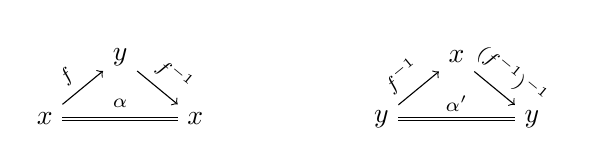
\begin{tikzpicture}[x=1.6em,y=1.4em]
  \node (y1) at (1.7,1.6) {$y$};
  \node (x1) at (0,0) {$x$};
  \node (x2) at (3.4,0) {$x$};
  \draw[->] (x1) -- node[above,sloped,pos=0.4]{$\scriptstyle f$} (y1);
  \draw[->] (y1) -- node[above,sloped,pos=0.6]{$\scriptstyle f^{-1}$} (x2);
  \draw[double] (x1) -- (x2);
  \node at (1.7,0.4) {$\scriptstyle\alpha$};
  \begin{scope}[shift={(7.6,0)}]
    \node (x3) at (1.7,1.6) {$x$};
    \node (y3) at (0,0) {$y$};
    \node (y4) at (3.4,0) {$y$};
    \draw[->] (y3) -- node[above,sloped,pos=0.4]{$\scriptstyle f^{-1}$} (x3);
    \draw[->] (x3) -- node[above,sloped,pos=0.6]{$\scriptstyle(f^{-1})^{-1}$} (y4);
    \draw[double] (y3) -- (y4);
    \node at (1.7,0.4) {$\scriptstyle\alpha'$};
  \end{scope}
\end{tikzpicture}
\end{center}

现在我们扩张已提升的映射 $E_{2}^{-}\cup_{E_{1}^{+}}E_{2}^{+}\to A$ 的数据，以
构造一个提升 $\tau\colon E_{3}^{-}\to B$ 的 3-\trSimplex{} $E_{3}^{-}\to A$；
做法是对\cref{cor:inner-fillings-complicial-set}之证明中的构造稍加修改。
我们定义一个复状内号角扩张
\begin{center}
\begin{tikzpicture}[x=1.6em,y=1.4em]
  \node (lt) at (0,1.3) {$\Lambda^{2}[4]$};
  \node (rt) at (3.6,1.3) {$A$};
  \node (lb) at (0,-1.3) {$\Delta^{2}[4]$};
  \node (rb) at (3.6,-1.3) {$B$};
  \draw[->] (lt) -- (rt);
  \draw[right hook->] (lt) -- (lb);
  \draw[->] (lb) -- node[below]{$\scriptstyle\tau\sigma^{2}$} (rb);
  \draw[->,dashed] (0.5,-1.0) -- (3.1,1.0);
  \draw[->>] (rt) -- node[right]{$\scriptstyle p$} (rb);
\end{tikzpicture}
\end{center}
使得第 2 面的提升即定义我们所求的\trSimplex{} $E_{3}^{-}\to A$。剩下的只是在
$\tau\sigma^{2}\colon\Delta^{2}[4]\to B$ 之上定义一个适当的号角
$\Lambda^{2}[4]\to A$。第 4 面是 $\alpha\sigma^{2}$。第 3 面经由沿一支
$\Lambda^{1}[3]$-号角作提升而构造：该号角的第 3 面是 $\alpha$、第 0 面是
$\alpha'$、第 2 面退化。记填充该号角所定义之面为 $\gamma$，第 1 面便经由填充
一支 $\Lambda^{0}[3]$-号角而构造，其第 2 面为 $\gamma$、第 1 面与第 3 面退化；
这一提升由\cref{lem:left-horn-filling-degenerate-edge}所容许。
第 0 面则经由填充
那支诸面均已描述完毕的 $\Lambda^{1}[3]$-号角而构造。填充该号角所定义的面是
替代 2-\trSimplex{} $\beta$——即 $\alpha'$ 的一个替代——它见证 $f$ 是其右逆
$f^{-1}$ 的右逆。这四枚 3-\trSimplex{}在 $\tau\sigma^{2}$ 之上定义了一个映射
$\Lambda^{2}[4]\to A$，其填充体定义了一块
\eqref{eq:replacement-3-simplex} 中所示形状的
3-\trSimplex{}面。这就定义了沿 $E_{1}^{-}\hookrightarrow E_{3}^{-}$ 所需的
提升。于是\cref{prop:inner-complicial-fibration-criterion}便完成了
「\trQuasiCategory{}之间的\trIsofibration{}皆是复状等价纤维化」的证明。
\end{proof}

有了这一结果，我们现在便可以把\trQuasiCategory{}之间的\trIsofibration{}类
整合进 D.3 节的诸结果之中，证明第 1 章中的\cref{prop:leibniz-exponential}与
\cref{prop:leibniz-exponential-trivial}——为方便起见在此重述。

\begin{proposition}\label{prop:leibniz-stability-isofibrations}
\begin{enumerate}[label=(\roman*)]
\item 介于「\trMonomorphism{} $i\colon X\hookrightarrow Y$ 与映射
  $\qcOne\hookrightarrow\qcInt$ 的\trLeibnizProduct」和「任一\trIsofibration{}
  $f\colon A\twoheadrightarrow B$」之间的任何提升问题都有解。
\item 若 $i\colon X\hookrightarrow Y$ 是\trMonomorphism{}且
  $f\colon A\twoheadrightarrow B$ 是\trIsofibration，则诱导的 Leibniz 指数
  映射 $i\widehat{\pitchfork}f\colon A^{Y}\twoheadrightarrow B^{Y}\times_{B^{X}}A^{X}$ 仍是\trIsofibration。
\item 若 $i\colon X\hookrightarrow Y$ 是\trMonomorphism{}且
  $f\colon A\qcTFib B$ 是\trTrivialFibration，则诱导的 Leibniz 指数映射
  $i\widehat{\pitchfork}f\colon A^{Y}\qcTFib B^{Y}\times_{B^{X}}A^{X}$ 仍是\trTrivialFibration。
\item 若 $i\colon X\hookrightarrow Y$ 属于由内号角包含与映射
  $\qcOne\hookrightarrow\qcInt$ \trCell{}式生成的类，且 $f\colon A\to B$ 是\trIsofibration，
  则诱导的 Leibniz 指数映射
  $i\widehat{\pitchfork}f\colon A^{Y}\qcTFib B^{Y}\times_{B^{X}}A^{X}$ 是\trTrivialFibration。
\end{enumerate}
\end{proposition}

\begin{proof}
只需在带标记单纯集中构造 (i) 的提升，然后遗忘标记。由%
\cref{lem:marked-anodyne-free-isomorphism}，当 $\qcInt$ 被赋予其自然的极大
标记时，$\qcOne\hookrightarrow\qcInt$ 是带标记\trAnodyneExtension。于是由%
\cref{prop:leibniz-marked-anodyne}，极小标记的\trMonomorphism{} $i$ 与该映射
的\trLeibnizProduct{}仍是带标记\trAnodyneExtension。由\cref{thm:isofibration-complicial-isofibration}，
一个\trIsofibration{}定义自然标记\trQuasiCategory{}之间的一个复状等价纤维化，
故所断言的提升存在。

(ii) 与 (iv) 两部分由 (i) 的结论与一个类似的结果——\cref{cor:leibniz-anodyne}
——得出：只需沿\trLeibnizProduct{}与 Leibniz 指数之间的双变量伴随转置提升问题。

(iii) 部分则由\cref{lem:leibniz-product-mono}中一个更容易的观察经类似的论证
得出：两个\trMonomorphism{}的\trLeibnizProduct{}仍是\trMonomorphism。
\end{proof}

\cref{thm:natural-marking-complicial}与%
\cref{thm:isofibration-complicial-isofibration}容许我们用复状技巧来求解
涉及\trQuasiCategory{}之间\trIsofibration{}的提升问题。本节的结果
提示：当涉及\trIsomorphism{}时，这些技巧特别富有成效。我们现在发展这一原理的
几个具体应用，它们将用于证明 1.1 节中最后一个尚缺的结果。

为此我们考虑一对余单纯带标记单纯集
\[
\Delta[\bullet]^{\sharp}\hookrightarrow\qcInt[\bullet]^{\sharp}
\qquad\in(\sSet^{+})^{\Delta}
\]
前者由极大标记\trSimplex{} $\Delta[n]^{\sharp}$ 给出，后者由对象
$0,1,\dots,n$ 上的极大标记可缩群胚 $\qcInt[n]^{\sharp}$ 给出。

\begin{lemma}\label{lem:natural-marking-reedy}
自然包含 $\Delta[\bullet]^{\sharp}\hookrightarrow\qcInt[\bullet]^{\sharp}$ 是
$(\sSet^{+})^{\Delta}$ 中诸 Reedy 单态的余单纯对象之间的一个 Reedy 单态射，
而且在\trVerity{}模型结构中它还是一个逐点\trWeakEquivalence。
\end{lemma}

\begin{proof}
当把 $\sSet^{+}$ 等同于其在 $\mathcal{S}et^{t\Delta^{\mathrm{op}}}$ 中的像时，
陈述的前一半由\cref{lem:unaugmentable-cosimplicial}的相对版本得出——该版本
作为\cref{ex:relative-unaugmentable}陈述——：诸「不可增广的」余单纯对象之间
的任何逐点\trMonomorphism，都是诸 Reedy 单态的余单纯对象之间的 Reedy 单态射。
由于面映射 $\delta^{0},\delta^{1}\colon\Delta[0]^{\sharp}\to\Delta[1]^{\sharp}$
与 $\delta^{0},\delta^{1}\colon\qcInt[0]^{\sharp}\to\qcInt[1]^{\sharp}$ 的%
\trEqualizer{}为空，$\Delta[\bullet]^{\sharp}$ 与 $\qcInt[\bullet]^{\sharp}$
二者都不可增广，于是我们得出结论：这些余单纯对象都是 Reedy 单态的，而自然包含
是 Reedy 单态射。

最后，为证 $\Delta[n]^{\sharp}\to\qcInt[n]^{\sharp}$ 是逐点\trWeakEquivalence，
我们诉诸\trTwoOfThreeProperty{}并论证：$\Delta[n]^{\sharp}$ 与
$\qcInt[n]^{\sharp}$ 二者都带标记同伦等价于 $\sSet^{+}$ 中的 $\qcOne$。其逆
等价由 $0\colon\qcOne\to\Delta[n]^{\sharp}$ 与
$0\colon\qcOne\to\qcInt[n]^{\sharp}$ 给出，而带标记\trHomotopy{}
$\Delta[n]^{\sharp}\times\Delta[1]^{\sharp}\to\Delta[n]^{\sharp}$ 与
$\qcInt[n]^{\sharp}\times\Delta[1]^{\sharp}\to\qcInt[n]^{\sharp}$ 则都由对象上
的映射 $(i,0)\mapsto 0$ 与 $(i,1)\mapsto i$ 定义。
\end{proof}

我们的意图是利用余单纯对象 $\Delta[\bullet]^{\sharp}$ 与
$\qcInt[\bullet]^{\sharp}$ 来「自由反转」单纯集 $K$ 的诸\trSimplex。为看出这
如何运作，再考虑由\trYonedaEmbedding{}定义的余单纯对象
$\Delta[\bullet]\in\sSet^{\Delta}$。由余 Yoneda 引理，\trWeightedColimit
$\operatorname{colim}_{K}\Delta[\bullet]\cong K$ 复得了原本的单纯集 $K$。
类似地，由于极大标记函子 $(-)^{\sharp}\colon\sSet\to\sSet^{+}$ 是%
\trLeftAdjoint，\trWeightedColimit{} $\operatorname{colim}_{K}\Delta[\bullet]^{\sharp}\cong K^{\sharp}$ 为单纯集 $K$ 配上了极大标记。最后，我们利用\trWeightedColimit{}二函子
定义 $\tilde{K}^{\sharp}\coloneqq\operatorname{colim}_{K}\qcInt[\bullet]^{\sharp}$。
这一函子的想法是：它把 $K$ 的每个 $n$-\trSimplex{}替换为 $\qcInt[n]^{\sharp}$
——「$n$ 个\trIsomorphism{}的一个同伦相干复合」。正如记号所提示的，
$\tilde{K}^{\sharp}$ 也是极大标记的。

\begin{proposition}\label{prop:free-inversion-trivial-cofibration}
对任何单纯集 $K$，自然映射 $K^{\sharp}\to\tilde{K}^{\sharp}$ 是\trVerity{}%
模型结构中的一个\textbf{平凡余纤维化}（trivial cofibration）。
\end{proposition}

\begin{proof}
任何单纯集 $K$ 在被视作 $\mathcal{S}et^{\Delta^{\mathrm{op}}}$ 的对象时都是
Reedy 单态的。于是，由\cref{cor:reedy-quillen-weighted-functors}，%
\trWeightedColimit{}函子
\[
\operatorname{colim}_{K}-\colon(\sSet^{+})^{\Delta}\to\sSet^{+}
\]
相对于 $(\sSet^{+})^{\Delta}$ 上的 Reedy 模型结构是左 Quillen 的。%
\cref{lem:reedy-factorization}与\cref{lem:natural-marking-reedy}证明
$\Delta[\bullet]^{\sharp}\hookrightarrow\qcInt[\bullet]^{\sharp}$ 是一个
Reedy 平凡余纤维化，于是正如所断言的，$K^{\sharp}\to\tilde{K}^{\sharp}$ 是
平凡余纤维化。
\end{proof}

我们把经由施用\trWeightedColimit{} $\operatorname{colim}_{K}\qcInt[\bullet]^{\sharp}$
并遗忘标记而定义的函子 $\widetilde{(-)}\colon\sSet\to\sSet$ 称作「自由反转
函子」（free-inversion functor）。

\begin{example}\label{exa:lifting-hc-composites}
\cref{prop:free-inversion-trivial-cofibration}可以施用于\trAnodyneExtension
$\Lambda^{1}[2]\hookrightarrow\Delta[2]$，以证明\trHomotopyCoherentIsomorphism{}%
的诸复合可以沿\trQuasiCategory{}的\trIsofibration{}被提升。据定义，
$\widetilde{\Delta[2]}\cong\qcInt[2]$，即顶点 $0$、$1$、$2$ 上的可缩群胚，故
我们对自由反转号角采用类似记号 $\widetilde{\Lambda^{1}[2]}\coloneqq\Lambda^{1}[\qcInt[2]]$。由于 $\Lambda^{1}[2]$ 系沿一个公共顶点粘合两支
1-\trSimplex{}而筑成，而自由反转函子保持余极限，我们看到
$\Lambda^{1}[\qcInt[2]]$ 是两个\trHomotopyCoherentIsomorphism{}之并——其一
介于 $0$ 与 $1$ 之间，另一介于 $1$ 与 $2$ 之间。给这些单纯集配上其极大标记，
则由施于方块
\begin{center}
\begin{tikzpicture}[x=1.7em,y=1.4em]
  \node (tl) at (0,1.3) {$\Lambda^{1}[2]^{\sharp}$};
  \node (tr) at (5.0,1.3) {$\Lambda^{1}[\qcInt[2]]^{\sharp}$};
  \node (bl) at (0,-1.3) {$\Delta[2]^{\sharp}$};
  \node (br) at (5.0,-1.3) {$\qcInt[2]^{\sharp}$};
  \draw[right hook->] (tl) -- (tr);
  \draw[right hook->] (tl) -- (bl);
  \draw[right hook->] (tr) -- (br);
  \draw[right hook->] (bl) -- (br);
\end{tikzpicture}
\end{center}
的\trTwoOfThreeProperty{}得出：包含
$\Lambda^{1}[\qcInt[2]]^{\sharp}\hookrightarrow\qcInt[2]^{\sharp}$ 是带标记
单纯集的一个平凡余纤维化。施用\cref{thm:isofibration-complicial-isofibration}，
我们得出结论：\trHomotopyCoherentIsomorphism{}的诸复合可以沿%
\trQuasiCategory{}之间的\trIsofibration{}被提升
\begin{center}
\begin{tikzpicture}[x=1.6em,y=1.4em]
  \node (lt) at (0,1.3) {$\Lambda^{1}[\qcInt[2]]$};
  \node (rt) at (4.4,1.3) {$A$};
  \node (lb) at (0,-1.3) {$\qcInt[2]$};
  \node (rb) at (4.4,-1.3) {$B$};
  \draw[->] (lt) -- (rt);
  \draw[right hook->] (lt) -- (lb);
  \draw[->] (lb) -- (rb);
  \draw[->] (rt) -- (rb);
  \draw[->,dashed] (0.5,-1.0) -- (3.9,1.0);
\end{tikzpicture}
\end{center}
\end{example}

一个类似的例子留作\cref{ex:horn-hc-isomorphisms-anodyne}。为完成对 1.1 节
所断言诸结果的验证，只剩下证明第 1 章中的%
\cref{prop:trivial-fibration-characterization}：

\begin{proposition}\label{prop:isofibration-characterizations}
对\trQuasiCategory{}之间的一个\trIsofibration{} $f\colon A\twoheadrightarrow B$，
下列诸条件等价：

\begin{enumerate}[label=(\roman*)]
\item $f$ 是\trTrivialFibration；
\item $f$ 既是\trIsofibration{}又是\trEquivalence；
\item $f$ 是一个\textbf{\trSplitFiberHomotopyEquivalence}：一个%
  \trIsofibration，它容许一个\trSection{} $s$，这个截面经由一个从
  $\mathrm{id}_{A}$ 到 $sf$ 的\trHomotopy{}而成为\trEquivalence{}逆，且该%
  \trHomotopy{}与 $f$ 复合后给出从 $f$ 到 $f$ 的常值\trHomotopy。
\end{enumerate}
\end{proposition}

\begin{proof}
对于 (i)$\Rightarrow$(ii)，观察到单纯形\trBoundary{}包含在\trCoproduct、\trPushout{}与
序列复合之下生成单纯集的诸\trMonomorphism（见\cref{lem:mono-epi-reedy-sset}），
于是第 1 章中的\eqref{eq:trivial-fibration}的提升性质蕴含：诸%
\trTrivialFibration{}对单纯集的一切\trMonomorphism{}都可提升，特别是对辨认出%
\trIsofibration{}类的那类\trMonomorphism。如此，\trTrivialFibration{}是%
\trIsofibration。由同一提升性质，每个\trTrivialFibration{}都容有一个截面
\begin{center}
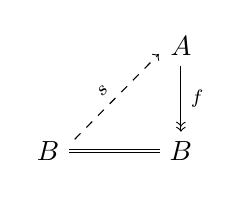
\begin{tikzpicture}[x=1.6em,y=1.4em]
  \node (a) at (3.0,1.5) {$A$};
  \node (b1) at (0,-1.2) {$B$};
  \node (b2) at (3.0,-1.2) {$B$};
  \draw[double] (b1) -- (b2);
  \draw[->,dashed] (0.6,-0.9) -- node[above,sloped,pos=0.45]{$\scriptstyle s$} (2.5,1.3);
  \draw[->>] (a) -- node[right]{$\scriptstyle f$} (b2);
\end{tikzpicture}
\end{center}
为证明 $s$ 定义 $f$ 的一个逆等价，观察到由常值\trHomotopy{}
$\pi\colon A\times\qcInt\to A$ 筑起的外矩形
\begin{center}
\begin{tikzpicture}[x=1.5em,y=1.5em]
  \node (tl) at (0,1.2) {$A+A$};
  \node (tr) at (5.6,1.2) {$A$};
  \node (bl) at (0,-1.2) {$A\times\qcInt$};
  \node (bm) at (3.4,-1.2) {$A$};
  \node (br) at (6.0,-1.2) {$B$};
  \draw[->] (tl) -- node[above]{$\scriptstyle(\mathrm{id}_{A},sf)$} (tr);
  \draw[right hook->] (tl) -- (bl);
  \draw[->,dashed] (1.7,-0.9) -- node[above,pos=0.6]{$\scriptstyle\alpha$} (5.3,1.0);
  \draw[->>] (tr) -- node[right]{$\scriptstyle f$} (br);
  \draw[->] (bl) -- node[below]{$\scriptstyle\pi$} (bm);
  \draw[->] (bm) -- node[above]{$\scriptstyle f$} (br);
  \node at (4.7,-0.45) {$\scriptstyle\sim$};
\end{tikzpicture}
\end{center}
交换，因为 $fsf=f$。该提升定义了一个介于 $\mathrm{id}_{A}$ 与 $sf$ 之间的%
\trHomotopy，完成了「\trTrivialFibration{}是\trEquivalence」的证明。而且
事实上注意：刚刚构造的这个\trEquivalence{}还是一个\trSplitFiberHomotopyEquivalence，
这就证明了 (i)$\Rightarrow$(iii)。

为证 (ii)$\Rightarrow$(iii)，设 $f$ 是带\trEquivalence{}逆 $g$ 的\trIsofibration。由下述%
\cref{lem:half-adjoint-equivalence}，从 $\mathrm{id}_{A}$ 到 $gf$ 的%
\trHomotopy{} $\alpha$ 与从 $fg$ 到 $\mathrm{id}_{B}$ 的\trHomotopy{} $\beta$
可以选取使之定义一个「半伴随等价」，意即：存在一个映射
$\Phi\colon A\times\qcInt[2]\to B$——其中 $\qcInt[2]$ 是三个对象上的可缩群胚
——其边缘由 $f\alpha$、$\beta f$ 与常值\trHomotopy{}
$\mathrm{id}_{f}\coloneqq f\pi$ 构成。\footnote{这与由带标记单纯集
$E_{3}^{-}$ 与 $E_{3}^{+}$ 所编码的半伴随等价概念相似但并不\trIsomorphism。}

施\cref{prop:leibniz-stability-isofibrations}(i) 于\trMonomorphism{}
$\varnothing\hookrightarrow B$，我们发现可以
沿 $f$ 提升介于 $fg$ 与 $\mathrm{id}_{B}$ 之间的\trHomotopy{} $\beta$
\begin{center}
\begin{tikzpicture}[x=1.7em,y=1.4em]
  \node (bt) at (0,2.4) {$B$};
  \node (a) at (5.0,2.4) {$A$};
  \node (bb) at (0,-1.2) {$B$};
  \node (bxi) at (3.4,-1.2) {$B\times\qcInt$};
  \node (br) at (6.6,-1.2) {$B$};
  \draw[->] (bt) -- node[above]{$\scriptstyle g$} (a);
  \draw[double] (bt) -- (bb);
  \draw[right hook->] (bt) -- (bxi);
  \node at (1.35,0.9) {$\scriptstyle i_{0}$};
  \draw[right hook->] (bb) -- (bxi);
  \node at (1.35,-1.75) {$\scriptstyle i_{1}$};
  \draw[->] (bxi) -- node[above]{$\scriptstyle\beta$} (br);
  \draw[->,dashed] (bb) -- node[above,sloped,pos=0.4]{$\scriptstyle s$} (a);
  \draw[->,dotted] (bxi) -- node[above,sloped,pos=0.55]{$\scriptstyle\gamma$} (a);
  \draw[->>] (a) -- node[right]{$\scriptstyle f$} (br);
\end{tikzpicture}
\end{center}
复合映射 $s$ 定义了 $f$ 的一个严格截面，而该提升定义了一个从 $g$ 到 $s$ 的%
\trHomotopy{} $\gamma$。施用\cref{prop:leibniz-marked-anodyne}、%
\cref{thm:isofibration-complicial-isofibration}与\cref{exa:lifting-hc-composites}，
我们可以求解提升问题
\begin{center}
\begin{tikzpicture}[x=1.9em,y=1.5em]
  \node (tl) at (0,2.2) {$A\times\Lambda^{1}[\qcInt[2]]$};
  \node (tr) at (10.2,2.2) {$A$};
  \node (ml) at (-1.8,-1.4) {$A\times\qcInt$};
  \node (mm) at (4.8,-1.4) {$A\times\qcInt[2]$};
  \node (mr) at (10.2,-1.4) {$B$};
  \node (ab) at (3.4,-3.9) {$A$};
  \draw[->] (tl) -- node[above]{$\scriptstyle(\alpha,\gamma f)$} (tr);
  \draw[right hook->] (tl) -- (mm);
  \draw[->] (ml) -- node[below]{$\scriptstyle\delta^{1}$} (mm);
  \draw[->] (mm) -- node[below]{$\scriptstyle\Phi$} (mr);
  \draw[->,dashed] (mm) -- node[above,sloped,pos=0.5]{$\scriptstyle\Psi$} (tr);
  \draw[->,dotted] (ml) -- node[above,sloped,pos=0.5]{$\scriptstyle\eta$} (tr);
  \draw[->] (ml) -- node[below,sloped]{$\scriptstyle\pi$} (ab);
  \draw[->] (ab) -- node[below,sloped]{$\scriptstyle f$} (mr);
  \draw[->>] (tr) -- node[right]{$\scriptstyle f$} (mr);
\end{tikzpicture}
\end{center}
该提升定义了一个从 $\mathrm{id}_{A}$ 到 $sf$ 的复合\trHomotopy{} $\eta$，使得
$f\eta=f\pi$ 是常值\trHomotopy。这份数据把 $f$ 展示为一个%
\trSplitFiberHomotopyEquivalence。

最后，对于 (iii)$\Rightarrow$(i)，注意\trSplitFiberHomotopyEquivalence{}的数据定义了一个
收缩图式
\begin{center}
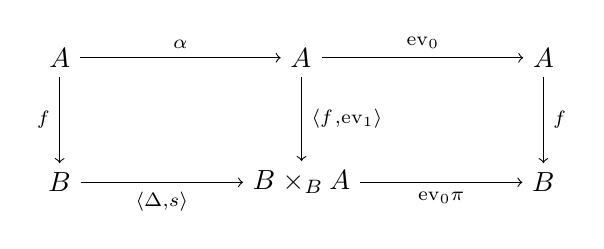
\begin{tikzpicture}[x=1.9em,y=1.5em]
  \node (a1) at (0,1.6) {$A$};
  \node (a2) at (4.6,1.6) {$A^{\qcInt}$};
  \node (a3) at (9.2,1.6) {$A$};
  \node (b1) at (0,-1.4) {$B$};
  \node (b2) at (4.6,-1.4) {$B^{\qcInt}\times_{B}A$};
  \node (b3) at (9.2,-1.4) {$B$};
  \draw[->] (a1) -- node[above]{$\scriptstyle\alpha$} (a2);
  \draw[->] (a2) -- node[above]{$\scriptstyle\mathrm{ev}_{0}$} (a3);
  \draw[->] (b1) -- node[below]{$\scriptstyle\langle\Delta,s\rangle$} (b2);
  \draw[->] (b2) -- node[below]{$\scriptstyle\mathrm{ev}_{0}\pi$} (b3);
  \draw[->] (a1) -- node[left]{$\scriptstyle f$} (b1);
  \draw[->] (a2) -- node[right]{$\scriptstyle\langle f^{\qcInt},\mathrm{ev}_{1}\rangle$} (b2);
  \draw[->] (a3) -- node[right]{$\scriptstyle f$} (b3);
\end{tikzpicture}
\end{center}
中央那个映射是 $\{1\}\hookrightarrow\qcInt$ 与\trIsofibration{} $f$ 的%
\trLeibnizCotensor，故由\cref{prop:leibniz-stability-isofibrations}它是一个%
\trTrivialFibration。由于\trTrivialFibration{}由一个右提升性质刻画，%
\cref{lem:right-lifting-closure}告诉我们：它们对\trRetract{}封闭。于是 $f$
正如所愿是一个\trTrivialFibration。
\end{proof}

\begin{lemma}\label{lem:half-adjoint-equivalence}
\trQuasiCategory{}的任何\trEquivalence
\begin{center}
\begin{tikzpicture}[x=1.6em,y=1.4em]
  \node (at) at (0,2.2) {$A$};
  \node (am) at (4.6,0.4) {$A$};
  \node (ax) at (0,-1.6) {$A\times\qcInt$};
  \node (ab) at (0,-3.8) {$A$};
  \node (b) at (4.6,-3.8) {$B$};
  \draw[double] (at) -- (am);
  \draw[right hook->] (at) -- (ax);
  \node at (-0.7,0.5) {$\scriptstyle i_{0}$};
  \draw[->] (ax) -- node[above]{$\scriptstyle\alpha$} (am);
  \draw[right hook->] (ab) -- (ax);
  \node at (-0.7,-2.6) {$\scriptstyle i_{1}$};
  \draw[->] (ab) -- node[below]{$\scriptstyle f$} (b);
  \draw[->] (b) -- node[right,pos=0.6]{$\scriptstyle g$} (am);
  \node at (8.6,0.4) {与};
  \begin{scope}[shift={(11.2,0)}]
    \node (bt) at (0,2.2) {$B$};
    \node (a) at (4.6,2.2) {$A$};
    \node (bxi) at (0,-0.4) {$B\times\qcInt$};
    \node (bb) at (0,-2.8) {$B$};
    \node (br) at (4.6,-2.8) {$B$};
    \draw[->] (bt) -- node[above]{$\scriptstyle g$} (a);
    \draw[right hook->] (bt) -- (bxi);
    \node at (-0.7,0.9) {$\scriptstyle i_{0}$};
    \draw[->] (bxi) -- node[above]{$\scriptstyle\beta$} (br);
    \draw[right hook->] (bb) -- (bxi);
    \node at (-0.7,-1.4) {$\scriptstyle i_{1}$};
    \draw[double] (bb) -- (br);
    \draw[->>] (a) -- node[right]{$\scriptstyle f$} (br);
  \end{scope}
\end{tikzpicture}
\end{center}
都可以扩张成\trQuasiCategory{}的一个\textbf{半伴随等价}（half adjoint
equivalence），即附带一个额外的相干\trHomotopy{} $\Phi\colon A\times\qcInt[2]\to B$，
其边缘由三个\trHomotopyCoherentIsomorphism{}组成：
\begin{center}
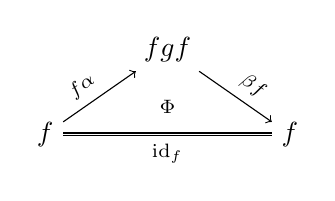
\begin{tikzpicture}[x=1.7em,y=1.4em]
  \node (t) at (2.6,1.8) {$fgf$};
  \node (bl) at (0,-0.4) {$f$};
  \node (br) at (5.2,-0.4) {$f$};
  \draw[->] (bl) -- node[above,sloped,pos=0.4]{$\scriptstyle f\alpha$} (t);
  \draw[->] (t) -- node[above,sloped,pos=0.6]{$\scriptstyle\beta f$} (br);
  \draw[double] (bl) -- node[below]{$\scriptstyle\mathrm{id}_{f}$} (br);
  \node at (2.6,0.3) {$\scriptstyle\Phi$};
\end{tikzpicture}
\end{center}
代价是替换\trHomotopy{} $\alpha$ 或 $\beta$ 之一。
\end{lemma}

其证明是对证明第 2 章中的\cref{prop:adjoint-equivalences}的那个 2-范畴式
论证所作的单纯式重释。

\begin{proof}
考虑如陈述中那般的\trQuasiCategory{}之\trEquivalence。由%
\cref{exa:lifting-hc-composites}，诸\trHomotopy{} $f\alpha$ 与 $\beta f$ 容有
某个复合，它由求解提升问题
\begin{center}
\begin{tikzpicture}[x=1.9em,y=1.5em]
  \node (tl) at (0,2.0) {$A\times\Lambda^{1}[\qcInt[2]]$};
  \node (tr) at (9.2,2.0) {$B$};
  \node (bl) at (-1.8,-1.6) {$A\times\qcInt$};
  \node (bm) at (4.8,-1.6) {$A\times\qcInt[2]$};
  \draw[->] (tl) -- node[above]{$\scriptstyle(f\alpha,\beta f)$} (tr);
  \draw[right hook->] (tl) -- (bm);
  \draw[->] (bl) -- node[below]{$\scriptstyle\delta^{1}$} (bm);
  \draw[->,dashed] (bm) -- node[above,sloped,pos=0.5]{$\scriptstyle\Psi$} (tr);
  \draw[->,dotted] (bl) -- node[above,sloped,pos=0.5]{$\scriptstyle\psi$} (tr);
\end{tikzpicture}
\end{center}
而定义。沿非恒同的对合 $\qcInt\to\qcInt$ 作限制，便定义了任何\trHomotopy{}的
逆，记作 $(-)^{-1}$。我们将把 $\alpha$ 替换为复合
$\alpha'\coloneqq g\psi^{-1}\cdot\alpha$——它由求解提升问题
\begin{center}
\begin{tikzpicture}[x=1.9em,y=1.5em]
  \node (tl) at (0,2.0) {$A\times\Lambda^{1}[\qcInt[2]]$};
  \node (tr) at (9.2,2.0) {$A$};
  \node (bl) at (-1.8,-1.6) {$A\times\qcInt$};
  \node (bm) at (4.8,-1.6) {$A\times\qcInt[2]$};
  \draw[->] (tl) -- node[above]{$\scriptstyle(\alpha,g\psi^{-1})$} (tr);
  \draw[right hook->] (tl) -- (bm);
  \draw[->] (bl) -- node[below]{$\scriptstyle\delta^{1}$} (bm);
  \draw[->,dashed] (bm) -- node[above,sloped,pos=0.5]{$\scriptstyle\Xi$} (tr);
  \draw[->,dotted] (bl) -- node[above,sloped,pos=0.5]{$\scriptstyle\alpha'$} (tr);
\end{tikzpicture}
\end{center}
而定义——并证明这一\trHomotopy{}与 $\beta$ 一起定义一个半伴随等价。

半伴随等价的见证由求解最后一个提升问题
\begin{center}
\begin{tikzpicture}[x=1.9em,y=1.5em]
  \node (tl) at (0,2.0) {$A\times\Lambda^{1}[\qcInt[3]]$};
  \node (tr) at (9.2,2.0) {$B$};
  \node (bl) at (-1.8,-1.6) {$A\times\qcInt[2]$};
  \node (bm) at (4.8,-1.6) {$A\times\qcInt[3]$};
  \draw[->] (tl) -- node[above]{$\scriptstyle\Gamma$} (tr);
  \draw[right hook->] (tl) -- (bm);
  \draw[->] (bl) -- node[below]{$\scriptstyle\delta^{1}$} (bm);
  \draw[->,dashed] (bm) -- (tr);
  \draw[->,dotted] (bl) -- node[above,sloped,pos=0.5]{$\scriptstyle\Phi$} (tr);
\end{tikzpicture}
\end{center}
而获得，它涉及沿 $\Lambda^{1}[\qcInt[3]]\hookrightarrow\qcInt[3]$ 的一个%
\trExtension——其余定义域是对象 $0$、$1$、$2$、$3$ 上的可缩群胚，其定义域是
含顶点 $1$ 的那三张 $\qcInt[2]$-面之并。这由\cref{ex:horn-hc-isomorphisms-anodyne}
所容许。

剩下的只是定义「同伦相干同构之号角」$\Gamma$ 的诸面，后者由诸%
\trHomotopyCoherentIsomorphism{}筑成
\begin{center}
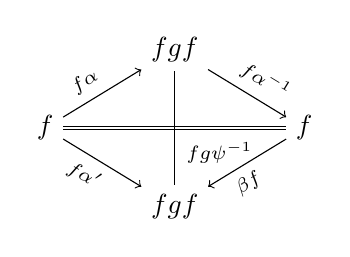
\begin{tikzpicture}[x=1.8em,y=1.5em]
  \node (t) at (2.6,1.9) {$fgf$};
  \node (l) at (0,0) {$f$};
  \node (r) at (5.2,0) {$f$};
  \node (b) at (2.6,-1.9) {$fgf$};
  \draw[->] (l) -- node[above,sloped,pos=0.4]{$\scriptstyle f\alpha$} (t);
  \draw[->] (t) -- node[above,sloped,pos=0.6]{$\scriptstyle f\alpha^{-1}$} (r);
  \draw[->] (l) -- node[below,sloped,pos=0.4]{$\scriptstyle f\alpha'$} (b);
  \draw[->] (r) -- node[below,sloped,pos=0.6]{$\scriptstyle\beta f$} (b);
  \draw[double] (l) -- (r);
  \draw (t) -- (b);
  \node at (3.5,-0.6) {$\scriptstyle fg\psi^{-1}$};
\end{tikzpicture}
\end{center}
第 3 面是 $f\Xi\colon A\times\qcInt[2]\to B$，而第 2 面是复合
\[
A\times\qcInt[2]\xrightarrow{\;A\times q\;}A\times\qcInt\xrightarrow{\;f\alpha\;}B
\]
其中 $q\colon\qcInt[2]\to\qcInt$ 是由 $0,2\mapsto 0$ 与 $1\mapsto 1$ 定义的
唯一映射。剩下的只是定义第 0 面。为此，我们首先沿另一支 $\mathcal{B}^{A}$ 中%
\trHomotopyCoherentIsomorphism{}的号角
$\Lambda^{1}[\qcInt[3]]\hookrightarrow\qcInt[3]$ 作\trExtension，如下图所绘
\begin{center}
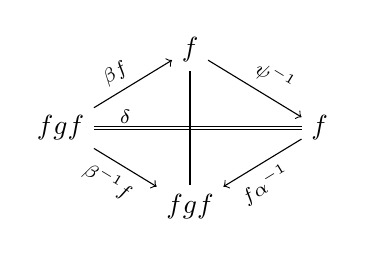
\begin{tikzpicture}[x=1.8em,y=1.5em]
  \node (t) at (2.6,1.9) {$f$};
  \node (l) at (0,0) {$fgf$};
  \node (r) at (5.2,0) {$f$};
  \node (b) at (2.6,-1.9) {$fgf$};
  \draw[->] (l) -- node[above,sloped,pos=0.4]{$\scriptstyle\beta f$} (t);
  \draw[->] (t) -- node[above,sloped,pos=0.6]{$\scriptstyle\psi^{-1}$} (r);
  \draw[->] (l) -- node[below,sloped,pos=0.4]{$\scriptstyle\beta^{-1}f$} (b);
  \draw[->] (r) -- node[below,sloped,pos=0.6]{$\scriptstyle f\alpha^{-1}$} (b);
  \draw[double] (l) -- (r);
  \node at (1.3,0.28) {$\scriptstyle\delta$};
  \draw (t) -- (b);
\end{tikzpicture}
\end{center}
这里第 0 面是 $\Psi^{-1}$，第 3 面是复合
\[
A\times\qcInt[2]\xrightarrow{\;A\times q\;}A\times\qcInt\xrightarrow{\;\beta f\;}B
\]
而第 2 面是复合
\[
A\times\qcInt[2]\xrightarrow{\;A\times d\;}A\times\qcInt[2]\times\qcInt
\xrightarrow{\;\Psi\times\qcInt\;}B\times\qcInt\xrightarrow{\;\beta\;}B
\]
其中 $d\colon\qcInt[2]\to\qcInt[2]\times\qcInt$ 是由 $0\mapsto(2,0)$、
$1\mapsto(2,1)$ 与 $2\mapsto(0,1)$ 定义的唯一映射。

这支号角的 $\delta^{1}$-面可用来定义最后一支 $\mathcal{B}^{A}$ 中%
\trHomotopyCoherentIsomorphism{}的号角
$\Lambda^{1}[\qcInt[3]]\hookrightarrow\qcInt[3]$，如下图所绘
\begin{center}
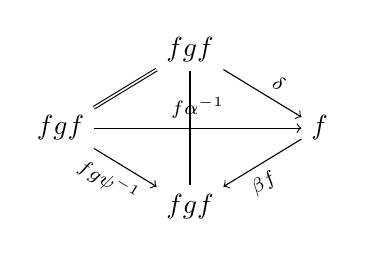
\begin{tikzpicture}[x=1.8em,y=1.5em]
  \node (t) at (2.6,1.9) {$fgf$};
  \node (l) at (0,0) {$fgf$};
  \node (r) at (5.2,0) {$f$};
  \node (b) at (2.6,-1.9) {$fgf$};
  \draw[double] (l) -- (t);
  \draw[->] (t) -- node[above,sloped,pos=0.6]{$\scriptstyle\delta$} (r);
  \draw[->] (l) -- node[above]{$\scriptstyle f\alpha^{-1}$} (r);
  \draw[->] (l) -- node[below,sloped,pos=0.4]{$\scriptstyle fg\psi^{-1}$} (b);
  \draw[->] (r) -- node[below,sloped,pos=0.6]{$\scriptstyle\beta f$} (b);
  \draw (t) -- (b);
\end{tikzpicture}
\end{center}
其第 3 面退化，其第 2 面是一个反转，交换刚定义的 $\delta^{1}$-面
$A\times\qcInt[2]\to B$ 的前两个顶点，而其第 0 面是复合
\[
A\times\qcInt[2]\xrightarrow{\;A\times c\;}A\times\qcInt[2]\times\qcInt
\xrightarrow{\;\Psi\times\qcInt\;}B\times\qcInt\xrightarrow{\;\beta\;}B
\]
其中 $c\colon\qcInt[2]\to\qcInt[2]\times\qcInt$ 是由 $0\mapsto(2,0)$、
$1\mapsto(0,0)$ 与 $2\mapsto(0,1)$ 定义的唯一映射。填充体定义出所求的第 0 面
\begin{center}
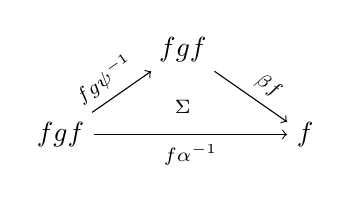
\begin{tikzpicture}[x=1.7em,y=1.4em]
  \node (t) at (2.6,1.8) {$fgf$};
  \node (bl) at (0,-0.4) {$fgf$};
  \node (br) at (5.2,-0.4) {$f$};
  \draw[->] (bl) -- node[above,sloped,pos=0.4]{$\scriptstyle fg\psi^{-1}$} (t);
  \draw[->] (t) -- node[above,sloped,pos=0.6]{$\scriptstyle\beta f$} (br);
  \draw[->] (bl) -- node[below]{$\scriptstyle f\alpha^{-1}$} (br);
  \node at (2.6,0.3) {$\scriptstyle\Sigma$};
\end{tikzpicture}
\end{center}
它补全了号角 $\Gamma\colon A\times\Lambda^{1}[\qcInt[3]]\to B$，而号角的填充
体便定义了 $\alpha'$ 与 $\beta$ 之间半伴随等价的见证。
\end{proof}

\subsection*{练习}

\begin{exercise}\label{ex:underlying-map-isofibration}
验证：自然标记\trQuasiCategory{}之间的一个复状等价纤维化所定义的底映射，是%
\trQuasiCategory{}之间的一个\trIsofibration。
\end{exercise}

\begin{exercise}\label{ex:horn-hc-isomorphisms-anodyne}
扩张\cref{exa:lifting-hc-composites}的结果，以证明：极大标记的「同伦相干同构
之 $\Lambda^{1}[\qcInt[3]]$-号角」
$\Lambda^{1}[\qcInt[3]]\hookrightarrow\qcInt[3]$ 是带标记\trAnodyneExtension——其余
定义域是顶点 $0$、$1$、$2$、$3$ 上的可缩群胚，而其定义域是由这四个顶点中凡含
顶点 $1$ 的三顶点子集所张成的三份 $\qcInt[2]$ 之并。
\end{exercise}

